%%%%%%%%%%%%%%%%%%%%%%%%%%%%%%%%%%%%%%%%%
% Beamer Presentation
% LaTeX Template
% Version 1.0 (10/11/12)
%
% This template has been downloaded from:
% http://www.LaTeXTemplates.com
%
% License:
% CC BY-NC-SA 3.0 (http://creativecommons.org/licenses/by-nc-sa/3.0/)
%
%%%%%%%%%%%%%%%%%%%%%%%%%%%%%%%%%%%%%%%%%

%----------------------------------------------------------------------------------------
%	PACKAGES AND THEMES
%----------------------------------------------------------------------------------------

\documentclass{beamer}

\mode<presentation> {

% The Beamer class comes with a number of default slide themes
% which change the colors and layouts of slides. Below this is a list
% of all the themes, uncomment each in turn to see what they look like.

%\usetheme{default}
%\usetheme{AnnArbor}
%\usetheme{Antibes}
%\usetheme{Bergen}
%\usetheme{Berkeley}
%\usetheme{Berlin}
\usetheme{Boadilla}
%\usetheme{CambridgeUS}
%\usetheme{Copenhagen}
%\usetheme{Darmstadt}
%\usetheme{Dresden}
%\usetheme{Frankfurt}
%\usetheme{Goettingen}
%\usetheme{Hannover}
%\usetheme{Ilmenau}
%\usetheme{JuanLesPins}
%\usetheme{Luebeck}
%\usetheme{Madrid}
%\usetheme{Malmoe}
%\usetheme{Marburg}
%\usetheme{Montpellier}
%\usetheme{PaloAlto}
%\usetheme{Pittsburgh}
%\usetheme{Rochester}
%\usetheme{Singapore}
%\usetheme{Szeged}
%\usetheme{Warsaw}
\usepackage{tikz}
% As well as themes, the Beamer class has a number of color themes
% for any slide theme. Uncomment each of these in turn to see how it
% changes the colors of your current slide theme.

%\usecolortheme{albatross}
%\usecolortheme{beaver}
%\usecolortheme{beetle}
%\usecolortheme{crane}
%\usecolortheme{dolphin}
%\usecolortheme{dove}
%\usecolortheme{fly}
%\usecolortheme{lily}
%\usecolortheme{orchid}
%\usecolortheme{rose}
%\usecolortheme{seagull}
%\usecolortheme{seahorse}
%\usecolortheme{whale}
%\usecolortheme{wolverine}

%\setbeamertemplate{footline} % To remove the footer line in all slides uncomment this line
%\setbeamertemplate{footline}[page number] % To replace the footer line in all slides with a simple slide count uncomment this line

%\setbeamertemplate{navigation symbols}{} % To remove the navigation symbols from the bottom of all slides uncomment this line
}
\logo{%
  \makebox[0.95\paperwidth]{%
    \tikz\node[opacity=0.4]{
\includegraphics[width=2cm,keepaspectratio]{mag.jpg}};%
    \hfill%
    \tikz\node[opacity=0.4]{
\includegraphics[width=2.5cm,keepaspectratio]{upb.png}};%
  }%
}
\usepackage{graphicx} % Allows including images
\usepackage{booktabs} % Allows the use of \toprule, \midrule and \bottomrule in tables

%----------------------------------------------------------------------------------------
%	TITLE PAGE
%----------------------------------------------------------------------------------------

\title[NICCI]{NICCI: Network-Informed Control -- Control-Informed Network} % The short title appears at the bottom of every slide, the full title is only on the title page

\author[Arun]{Dr. Arunselvan Ramaswamy %\\ \&
 } % Your name
\institute[Paderborn University] % Your institution as it will appear on the bottom of every slide, may be shorthand to save space
{
Dept. of Electrical Engineering and Information Technology, \\
Paderborn University \\ % Your institution for the title page
\textit{arunselvan.ramaswamy@upb.de}\\
%\vspace*{.1in}
%Whose involved
}
\date{October 19, 2017} % Date, can be changed to a custom date
% \usebackgroundtemplate{%
% \tikz[overlay,remember picture] \node[opacity=0.2, at=(current page.center)] {
%    
\includegraphics[height=.3\paperheight,width=.2\paperwidth]{upb.jpg}};
% }
\begin{document}
% \usebackgroundtemplate{
% \tikz\node[opacity=0.2] 
\includegraphics[width= .5 \paperwidth]{upb.png}} 
\begin{frame}
\titlepage % Print the title page as the first slide
\end{frame}

\begin{frame}
\frametitle{Overview} % Table of contents slide, comment this block out to remove it
\tableofcontents % Throughout your presentation, if you choose to use \section{} and \subsection{} commands, these will automatically be printed on this slide as an overview of your presentation
\end{frame}
\section{Networked control systems}
\begin{frame}
 \frametitle{Networked control systems}
%  \begin{block}{Stochastic approximation algorithms}
%  \end{block}
\begin{columns}
\begin{column}{0.5\textwidth}
\begin{figure}
\centering
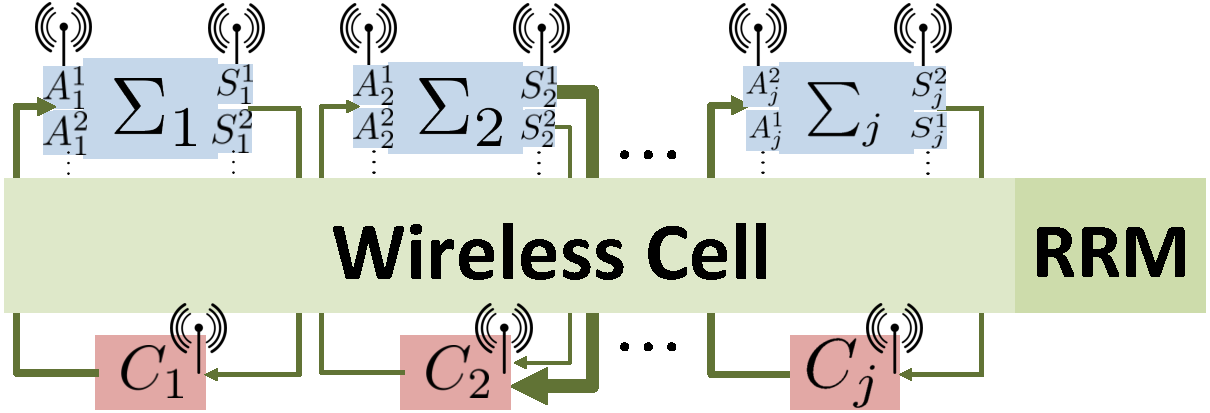
\includegraphics[width=0.8\textwidth]{CSRM.pdf}
% \caption{{\footnotesize Source: \href{https://heemels.tue.nl/research/networked-control}{www.heemels.tue.nl}}} 
\label{fig1}
\end{figure}
\end{column}
\begin{column}{0.5\textwidth}  %%<--- here
\begin{figure}
\centering
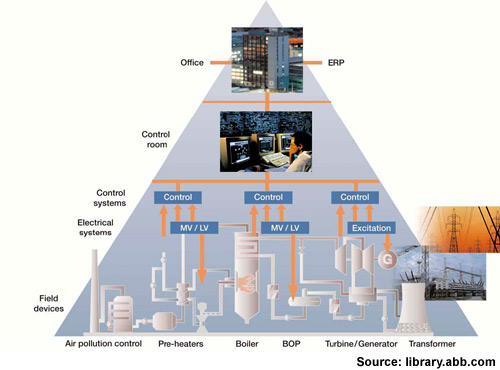
\includegraphics[width=0.75\textwidth]{ncs3}
\caption{{\footnotesize Figure illustrating modularity}} 
\label{fig3}
\end{figure}
\end{column}
\end{columns}
\begin{itemize}
 \item Large scale, modular, distributed systems.
 \item Components share resources such as communication channels, computational resources.
 \item Controllers use both local (immediate) and global (delayed) information.
 \item Controllers act asynchronously {\color{blue}(run on their own clocks)}.
\end{itemize}
\end{frame}
\begin{frame}
 \frametitle{Resource aware control -- control aware resource}
 \begin{itemize}
  \item Due to the large scale of systems being considered, resources such as communication
  channels and processors may be constrained.
  \item[]
  \item RRM is responsible for ``sequential decision making'' with regards to communication.
  \item `Quality of control' and `RRM decisions' are mutually influential.
  \item There may be other resource managers, eg. computational resources.
 \end{itemize}
  \begin{block}
   {\color{violet} Goal: Develop and analyze algorithms for distributed control of large-scale
  systems (process and radio) under resource constraints.}
  \end{block}
\end{frame}
% \begin{frame}
%  \frametitle{Dynamic Programming and Optimal Control}
%  \begin{itemize}
%   \item Discrete time dynamical systems: State (finite) evolves according to control (finite) taken and 
%   transition probabilities.
%   \item Rules by which controls are picked are called {\color{orange}policies} 
%   or {\color{orange}feedback control policies}.
%   \item DP principle is based on the Bellman equation:
%   \[
%     J^*(i) = \min \limits_{\pi} E_\pi \left[ g(i,\pi(i),j)+ J^*(j) \right]
%   \]
%   \item Popular DP algorithms: Value iteration, Policy iteration, Policy gradient descent, Q-learning, Temporal
%   difference learning.
%   \item {\color{purple}Goal: DP for optimal control in the setting of distributed large-scale systems
%   with lossy, delayed communications.}
%  \end{itemize}
%  \end{frame}
 
\section{Chapter I: Radio Resource Management}
\begin{frame}
\centerline{\textbf{Chapter I: Radio Resource Management (RRM)}}
% \begin{center}
%  Prof. Holger Karl
% \end{center}

\end{frame}
\begin{frame}
  \frametitle{RRM for short-term dependability}
  \begin{itemize}
  
  \item Let's start with the RRM-side.
  \item[]
  \item Issue:  Dependable communication 
    \begin{itemize}
    \item Over fading channels.
    \item[]
    \item With short deadlines.
    \item[]
    \item And limited  diversity (related to number of stochastically independent channels).
    \item[]
    \item But with some limited prediction (deadline longer than
      coherence time).
    \end{itemize}
 \item[]
 \item Bad combination -- but what is achievable? 
  \end{itemize}
\end{frame}

\begin{frame}
  \frametitle{First approach: Markov model for fading channel}

  \begin{itemize}
  \item Markov chain extracted from  Clark's model 
    \begin{itemize}
    \item States correspond to Signal-to-noise ratio (SNR) regions
    \item Which in turn correspond to
      Modulation/Coding Scheme (MCS) performance at negligible transmission error rate.
    \end{itemize}
    \item[]
  \item Under these assumptions: 
    \begin{itemize}
    \item What is the \emph{time-limited capacity}, for an acceptable model prediction
      error?
      \begin{itemize}
      \item In a sense: Real-time version of outage capacity. 
      \end{itemize}
    \item Can it be communicated to a control system as options? 
    \end{itemize}
    \item[]
  \item Formulate as Markov reward (no.\ of bits that can be transmitted) model.
  \end{itemize}
\end{frame}
\begin{frame}
  \frametitle{Time-limited capacity: First hints at results}
  \begin{itemize}
  \item What is the (normalized, per time slot) {\color{blue}available capacity}
  for {\color{blue}different acceptable error rates} over {\color{blue}increasing number of time slots}?
  \item \textbf{Observation}: Clear dependence on acceptable error rate. 
  \end{itemize}
  
  \begin{center}
    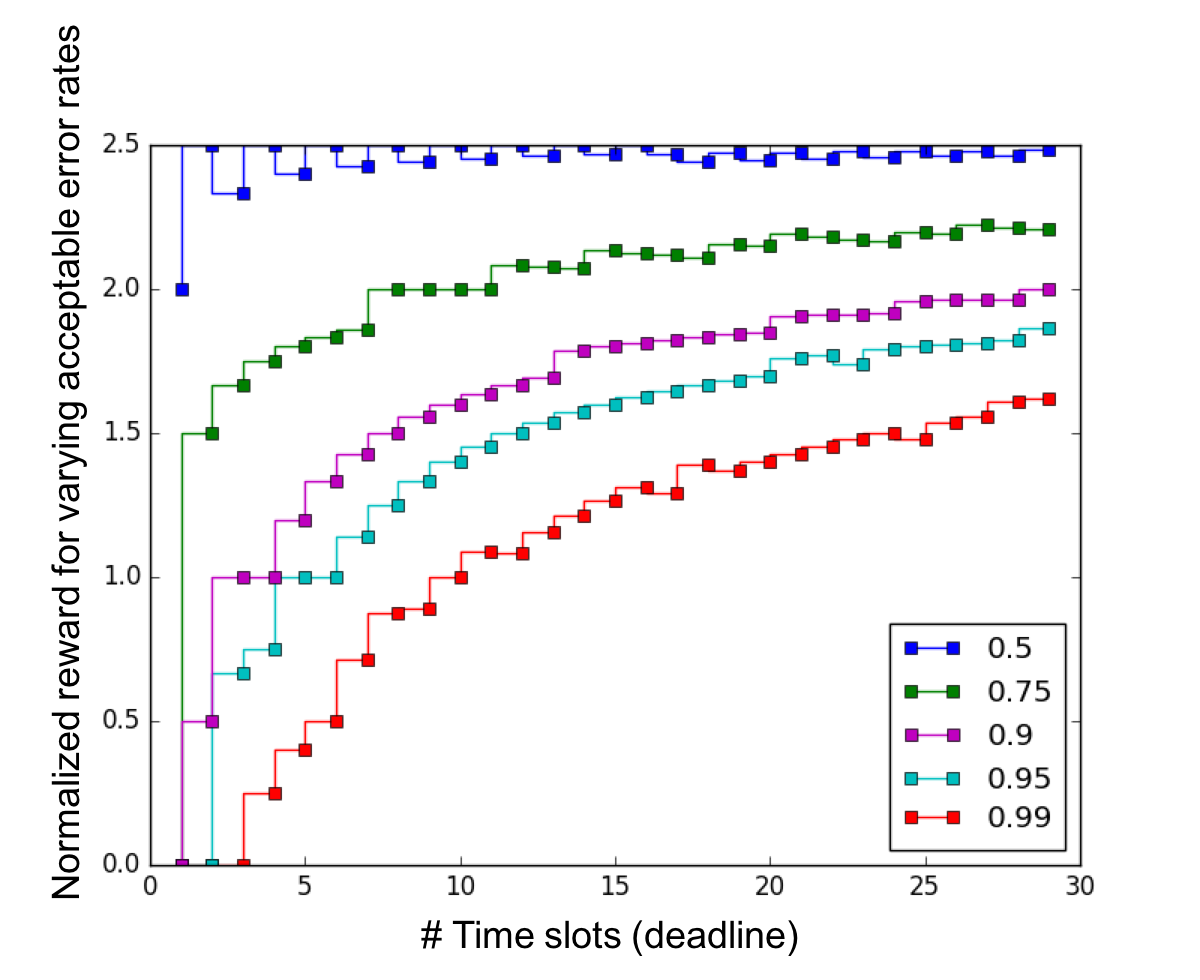
\includegraphics[width=0.6\columnwidth]{rewards-correlated}
  \end{center}
\end{frame}

\begin{frame}
  \frametitle{Closing Remarks: Influencing factors in time-limited capacity}
  \begin{center}
    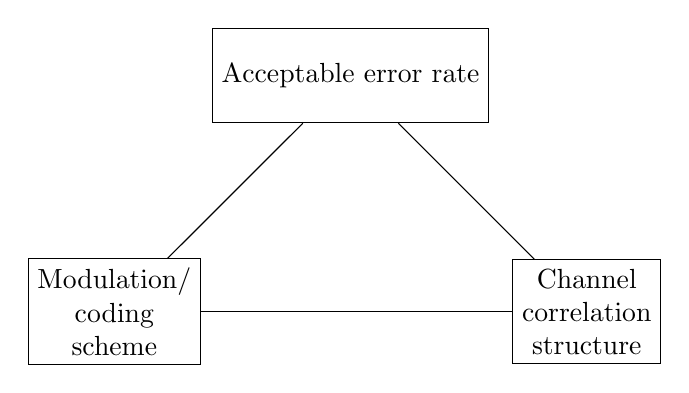
\begin{tikzpicture}[box/.style = {draw, minimum height=12mm,
        align=center}]
      \node (aer) [box] at (3,3) {Acceptable error rate}; 
      \node (mcs) [box] at (0,0)  {Modulation/\\coding\\scheme}; 
      \node (ccs) [box] at (6,0)  {Channel \\correlation\\ structure}; 
      \draw[] (aer) -- (mcs); 
      \draw[] (aer) -- (ccs); 
      \draw[] (mcs) -- (ccs); 
    \end{tikzpicture}
  \end{center}
\end{frame}
\section{Chapter II: Output Feedback MPC with Scheduled Communications}
\begin{frame}
\centerline{\textbf{Chapter II: Output Feedback MPC with Scheduled Communications}
}
% \begin{center}
%  Markus K\"{o}gel and Prof. Rolf Findeisen
% \end{center}
\end{frame}
\begin{frame}
 \frametitle{Motivation and setup}
 \begin{figure}
\centering
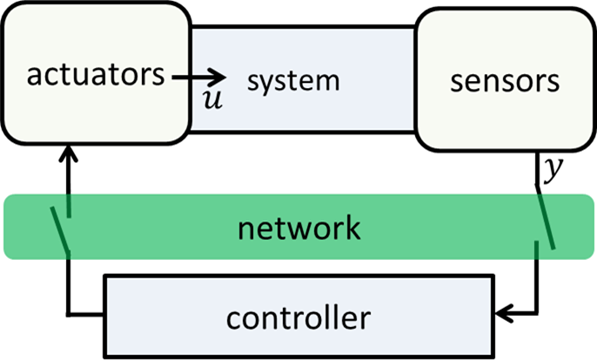
\includegraphics[width=0.4\textwidth ]{clc.png}
% \caption{{\footnotesize Source: \href{https://heemels.tue.nl/research/networked-control}{www.heemels.tue.nl}}} 
% \label{fig1}
\end{figure}
 \begin{itemize}
  \item Dynamics: (i) unknown, but bounded uncertainties, (ii) discrete time, linear systems, (iii) noisy measurements.
  \item Communications networks: (i) reliable, (ii) limited communication. %, \textit{for example}  either \textbf{to actuator} \textit{or}   \textbf{from sensor}.
  \item Challenge: When/what/where to send to maximize  performance.
 \end{itemize}
\end{frame}
\begin{frame}
\frametitle{Communication scheduling - basic idea} 

\begin{itemize}\item \textbf{Toy example:}
\begin{itemize}
 \item   either sensor sends $y_k$ or controller sends $u_k$. 
  \item[] If no data is received, then actuator uses $u_k = u_{k-1}$.
	\item Question: when to sense and when to actuate? %Benefit of sending extra data? 
 \end{itemize}

	\item \textbf{
  Solution approach to optimize communication:}
	\begin{itemize}
\item consider fixed communication schedule  
\item compare  schedules, select the one with best  performance
\end{itemize}	
	Requires: Efficient performance evaluation, avoid controller tuning.
\end{itemize}

\begin{figure}
\centering
\vspace*{-.2in}
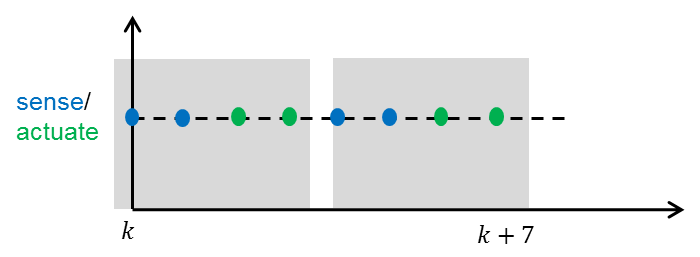
\includegraphics[width=0.7\textwidth ]{timing2.png}\\
  {{\footnotesize Communication schedule}} 
% \label{fig1}
\end{figure} 
\end{frame}
\begin{frame}
 \frametitle{Problem setup and contribution  }
 \begin{itemize} 
  \item \textbf{Considered system class:} \\(i) LTI system with process noise, $x_{k+1} = A x_k + B u_k + w_k$,  $w_k \in \mathbb{W}$.\\
  (ii) State and input constraints: $x_k\in\mathbb{X}$ and $u_k\in\mathbb{U}$.\\
  (iii) Noisy measurements: $y_k = C x_k + v_k, \ v_k \in \mathbb{V}$.
    \item \textbf{Robust output feedback MPC} (model predictive control):
  \begin{itemize}
   \item \textbf{Tube approach:} Decompose dynamics into (a)  nominal system + MPC
   and (b) error systems +  \textbf{ ``tube controller''}.
   \item \textbf{Performance:} For example  worst case optimal set-point tracking: 
  \end{itemize}  
	$\Rightarrow$    ``Minimize''  distance from optimality - tune ``tube controller''! 
\item  \textbf{Contribution:}
\begin{itemize}  
\item 
Automated, efficient optimal controller design  for given schedule
 \item Allows for comparison between different schedules.
 \item Guarantees on closed loop behavior (constraint satisfaction, stability). 
\end{itemize}
\end{itemize}
 

\end{frame}

%%%%%%%%%%%%%%%%%%%%%%%%%%%%%%%%%%%%%%%%%%%%%%%%%%%%%%%%%%%%%%%%%%%%%%%%%%%%%%%%%%%%%%%%%%%%%%%%%%%%%
% \begin{frame}
% \frametitle{Diversion: Dynamic programming algorithms \cite{p2}}
% \begin{block}{Value iteration}
%  $T(J)(i) := min_{u} E \left( g(i,u,j) + J(j) \mid i,u \right)$ is the Bellman operator 
%  for the {\color{orange} stochastic shortest path problem}
%  {\color{orange}(contractive w.r.t. to some norm)}.\\
%  {\color{purple}Algorithm: $J_{n+1} = J_{n} + a(n) \left( TJ_n - J_n + M_{n+1}\right)$}. \\
% \end{block}
% \begin{block}{Q-Learning}
%  $Q^*(i,u) := \sum \limits_j p(i,j)(u) \left(g(i,u,j) + \min \limits_{v \in U(j)} Q^*(j,v) \right)$
%  is the Bellman equation for Q-factors.\\
%  {\color{purple}Algorithm:$Q_{k+1} = Q_{k} + a(n) \left(F(Q_k, \psi_k) - Q_k \right) $}, where
%  $F(Q_k, \psi_k) = g(i,u, \psi^{iu}_k) + \min \limits_{v \in U(\psi_{iu})} Q(\psi^{iu}_k,v)$ and
%  $P(\psi^{iu}_k = j) = p_{ij}(u)$.
% \end{block}
% \begin{itemize}
%  \item Policy gradient descent, $TD(\lambda)$, actor-critic algorithm (policy iteration).
% \end{itemize}
% \end{frame}
%%%%%%%%%%%%%%%%%%%%%%%%%%%%%%%%%%%%%%%%%%%%%%%%%%%%%%%%%%%%%%%%%%%%%%%%%%%%%%%%%%%%%%%%%%%%%%%%%%%%%%%
% \section{Getting back to distributed control of large-scale systems}
\section{Chapter III: Reinforcement Learning Approach}
\begin{frame}
\centerline{\textbf{Chapter III: Reinforcement Learning Approach}}
% \begin{center}
%  Arun Ramaswamy and Prof. Daniel E. Quevedo
% \end{center}

\end{frame}
\begin{frame}
 \frametitle{Multi-agent systems perspective}
 \begin{figure}
\centering
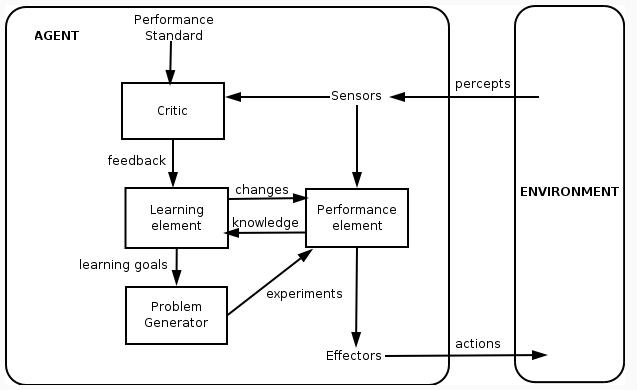
\includegraphics[height= .3 \textheight, width=.6\textwidth]{ncs2}
\caption{{\footnotesize Point-of-view of one agent, one of many! (source: wikipedia)}} 
\label{fig2}
\end{figure}
\vspace*{-.3in}
\begin{itemize}
 \item RRM and controllers are viewed as autonomous agents.
 \item These agents interact with a stochastic environment.
 \item Model of this environment is {\color{blue} unknown}.
 \item Requirements for offline algorithms: {\color{blue}availability of labeled data}. 
 \item In case of online algorithms: {\color{blue} learn the model on-the-go}.
\end{itemize}
\end{frame}

\begin{frame}
  \frametitle{Motivation: Dynamic programming approach}
  \begin{itemize}
  \item {\color{blue} Develop and analyze approximate, asynchronous value iteration and 
  policy gradient algorithms}.
%   \item Consider a re-engineering of Value Iteration and Policy Gradient Descent to solve our problems.
  \item Value iteration is given by $J_{n+1} = T J_n$, where
  $TJ(i) := \min \limits_{\pi} E_\pi \left[ g(i,\pi(i),j)+ J(j) \right]$ is the Bellman operator.
  \item We mutate its stochastic iterative counterpart:
   \[
    {\color{violet}J_{n+1} = J_{n} + a(n) \left( TJ_n - J_n + M_{n+1}\right).}
   \]
   \item We also mutate policy gradient descent given by:
   \[
   {\color{violet}\theta_{n+1} = \theta_n  - a(n) \left[ \nabla_\theta \pi(\theta) + M_{n+1} \right].}
   \]
   \item {\color{blue}Summary}: Re-engineer for large-scale distributed asynchronous systems
   with lossy, delay-prone communication systems.
  \end{itemize}
 \end{frame}
% \begin{frame}
% \frametitle{The Hateful 5}
%  \begin{itemize}
%    \item Large-scale $\implies$ {\color{violet} DP will suffer from Bellman's curse of dimensionality}. Need
%    to use an approximation operator.
%    \item Approximation operators $\implies$ {\color{violet} DP becomes unstable (algorithm may go out of bounds)}.
%    Stability conditions!
% %   \item Distributed $\implies$ {\color{violet}hence each agent is responsible for updating his/her state(s)}.
%   \item Asynchronous $\implies$ {\color{violet} each agent runs on a different clock (inter action time
%   is controller dependent)}. Need to capture relative clock speed.
%   \item Error prone communications $\implies$ {\color{violet} Information may be lost and out of order.
%   The delays may be unbounded}. Need to deal with errors arising due to this.
%   \item Resource constraints $\implies$ {\color{violet} Only a subset of agents are active. Only a subset
%   of agents are communicating}. Need to figure out causal relationships between agents.
%  \end{itemize}
% \end{frame}
%%%%%%%%%%%%%%%%%%%%%%%%%%%%%%%%%%%%%%%%%%%%%%%%%%%%%%%%%%%%%%%%%%%%%%%%%%%%%%%%%%%%%%%%%%%%%%%%%%%%%%%%%%%
%%%%%%%%%%%%%%%%%%%%%%%%%%%%%%%%%%%%%%%%%%%%%%%%%%%%%%%%%%%%%%%%%%%%%%%%%%%%%%%%%%%%%%%%%%%%%%%%%%%%%%%%%%%
%%%%%%%%%%%%%%%%%%%%%%%%%%%%%%%%%%%%%%%%%%%%%%%%%%%%%%%%%%%%%%%%%%%%%%%%%%%%%%%%%%%%%%%%%%%%%%%%%%%%%%%%%%%
%%%%%%%%%%%%%%%%%%%%%%%%%%%%%%%%%%%%%%%%%%%%%%%%%%%%%%%%%%%%%%%%%%%%%%%%%%%%%%%%%%%%%%%%%%%%%%%%%%%%%%%%%%%
% \section{Approximate asynchronous Value Iteration}
\begin{frame}
 \frametitle{Approximate asynchronous Value Iteration}
 \begin{block}{Re-engineered value iteration algorithm} {\footnotesize
$J_{n+1}(i) = J_n(i) + {\color{red} a(\nu(i,n))} {\color{orange} I\{i \in Y_n\}} \times
\left( {\color{purple}\mathcal{A}}T (J_{n - \tau_{1i}(n)}(1), \ldots, 
J_{n - \tau_{di}(n)}(d))(i) - J_n(i) + M_{n+1}(i) \right)$.}
\end{block}
\begin{itemize}
\item $\nu(i,n)$ is the number of times that agent $i$ was active till time $n$.
 \item $Y_n \subseteq \{1, \ldots, d\}$ denotes the active agents at time $n$.
 \item $0 \le \tau_{ij}(n) \le n$. Delay faced by {\color{blue}agent j}, at time $n$, in receiving information from 
 {\color{blue}agent i}.
 \item $\mathcal{A}$ is the approximation operator {\color{orange} 
 (obtained as a consequence of a supervised learning algorithm)}.
 \item $M_{n+1}$ is the Martingale difference noise.
\end{itemize}
\end{frame}
% \begin{frame}
% \frametitle{A Closer Look}
% \begin{block}{Recall} 
% $J_{n+1}(i) = J_n(i) + {\color{red} a(\nu(i,n))} {\color{orange} I\{i \in Y_n\}} \times$
% $\left( {\color{purple}\mathcal{A}}T (J_{n - \tau_{1i}(n)}(1), \ldots, 
% J_{n - \tau_{di}(n)}(d))(i) - J_n(i) + M_{n+1}(i) \right)$.
% \end{block}
% \begin{itemize}
%  \item The RRM may try to maximize 
%  ({\color{orange}using some sequential decision making algorithm such as MAB(andit)}) the communications throughput along with
%  \[
%   \min \limits_{ij} \frac{\# \text{ of times agents $i$ and $j$ have communicated till stage $n$}}{n}
%  \]
% \item Agent $i$ needs to be dormant for the next $10$ stages and doesn't need any new information
% from other agents.
% \item Will affect the ``$Y_n$-process'' and the time delays $\tau_{ij}(n)$. 
% \end{itemize}
% \end{frame}
% \section{Approximate asynchronous Policy Gradient Descent (AAPGD)}
\begin{frame}
 \frametitle{Approximate asynchronous Policy Gradient Descent (AAPGD)}
 \begin{itemize}
  \item Basic idea of PGD is the existence of a parameterization $\pi(\theta)$ 
  {\color{purple}(policy objective function)}, Sutton et. al. \footnote{
  {\footnotesize \color{purple} R.S. Sutton et al. "Policy gradient methods for reinforcement learning with function approximation." 
 Advances in neural information processing systems. 2000.}
  }. 
  The goal is to find
  a local minimizer $\hat{\theta}$.
  \end{itemize}
  \begin{block}{Re-engineered policy gradient descent}{\footnotesize
   $\theta_{n+1}(i) = \theta_n (i)  - a(\nu(i,n)) I\{ i \in Y_n\} \left(
    {\color{red}\mathcal{A}}\nabla_\theta \pi_i(\theta_{n - \tau_{1i}(n)}(1), \ldots, 
\theta_{n - \tau_{di}(n)}(d)) + M_{n+1} \right)
    $.}
  \end{block}
  \begin{itemize}
%    \item Forced mini-batch stochastic gradient descent.
   \item It allows for ``finite-difference'' implementations of GD using SPSA or SPSA-C
   (simultaneous perturbations stochastic approximations).
   \item In the above equation, we may replace the {\color{purple}gradient terms} with {\color{purple} sub-gradients}, 
   our analysis still carries through, verbatim.
    \item {\color{purple}While approximate asynchronous value iteration is offline, AAPGD is online}.
  \end{itemize}
\end{frame}
% \begin{frame}
%  \frametitle{The to-do list}
%  \begin{itemize}
%   \item Hope we have agreed upon the re-engineered value iteration and policy gradient descent algorithms.
%   \item We need to analyze where these algorithms converge.
%   \item We need to check if the use of approximation operators affect the stability of the algorithms.
%   \item Approximate DP usually leads to sub-optimal results. We need to quantify them.
%   \item Asynchronous updates usually affect the long-term behavior of the control algorithm.
%   \begin{itemize}
%    \item Can we enforce causal relations without affecting asynchronicity.
%    \item Would balanced step-sizes help?
%   \end{itemize}
%  \end{itemize}
% 
% \end{frame}

% \section{Stochastic Approximation Algorithms}
% \begin{frame}
%  \frametitle{Analysis: ODE Method \cite{p10}}
%  \begin{itemize}
%   \item The reason we considered stochastic iterative DP is because they have the following model-free 
%   structure:
%   \begin{equation}
%   \label{saae1}
%    x_{n+1} = x_n + a(n) \left( h(x_n) + M_{n+1} \right),
%   \end{equation}
%    \item ODE Method: Provides conditions under which long-term behavior of the above is identical to that of
%    $\dot{x}(t) = h(x(t))$.
%    \item In our case, due to approximation operators, $h$ of (\ref{saae1}) is {\color{red}set-valued}.
%    \item In the case of simple VI,
%    $J_{n+1} = J_{n} + a(n) \left( TJ_n - J_n + M_{n+1}\right)$, it can be shown that we may
%    study the long-term behavior of $\dot{J}(t) = TJ(t) - J(t)$.
%   \end{itemize}
% \end{frame}
%%%%%%%%%%%%%%%%%%%%%%%%%%%%%%%%%%%%%%%%%%%%%%%%%%%%%%%%%%%%%%%%%%%%%%%%%%%%%%%%%%%%%%%%%%%%%%%%%%%%%%%
%%%%%%%%%%%%%%%%%%%%%%%%%%%%%%%%%%%%%%%%%%%%%%%%%%%%%%%%%%%%%%%%%%%%%%%%%%%%%%%%%%%%%%%%%%%%%%%%%%%%%%%
%%%%%%%%%%%%%%%%%%%%%%%%%%%%%%%%%%%%%%%%%%%%%%%%%%%%%%%%%%%%%%%%%%%%%%%%%%%%%%%%%%%%%%%%%%%%%%%%%%%%%%%
% \section{Our results}
% \begin{frame}
%  \frametitle{A more generalized asynchronous, approximate iterative scheme}
%   \begin{block}
% {\color{blue}   $x_{n+1}(i) = x_n(i)  + a(\nu(i,n))I\{ i \in Y_n\} \times$ $\left( \mathcal{A}h_i(x_{n - \tau_{1i}(1)}, \ldots, x_{n - \tau_{1i}(d)}) 
%    + M_{n+1}(i) \right)$, where}
%   \end{block}
% \begin{itemize}
%  \item $\mathcal{A}h(x) \in h(x) + \overline{B}_\epsilon(0)$ for all $x$'s ``encountered'' and
%  $\epsilon > 0$ fixed.
%  \begin{itemize}
%   \item Typically $\mathcal{A}$ is a supervised learning algorithm used to find an approximation of
%   $T$ by minimizing least square errors w.r.t. to some norm.
%  \end{itemize}
%  \item $\nu(i,n) = \sum \limits_{m=0}^n I\{ i \in Y_m\}$.
%  \begin{itemize}
%   \item $\nu(i,n)$ is the number of times that agent $i$ was active up to time $n$. 
%  \end{itemize}
%  \item $\sum_n a(n) = \infty$ and $\sum_n a(n)^2 < \infty$, is the chosen step-size sequence.
% \end{itemize}
% \end{frame}
% \begin{frame}
%  \frametitle{Analysis, stage 0: Assumptions}
%  \begin{itemize}
%   \item {\color{blue}   $x_{n+1}(i) = x_n(i)  + a(\nu(i,n))I\{ i \in Y_n\} \times$ 
%   $\left( \mathcal{A}h_i(x_{n - \tau_{1i}(1)}, \ldots, x_{n - \tau_{di}(d)}) 
%    + M_{n+1}(i) \right)$}.
%    \item Causal assumptions on local-clocks: $\liminf \limits_{n \to \infty} \frac{\nu(i,n)}{n} > 0$.
%    {\color{orange}Agents are active comparably often.}
%    \item Agent $i$ knows $x_{n - \tau_{ji}(n)}(j)$ but not $x_m(j)$ for $m > n - \tau_{ji}(n)$. Maybe the
%    agent does know some of them but does not realize they are more recent.
%    \item The $\{Y_n\}_{n \ge 0}$ process is controlled by RRM and possibly other players.
%    \item {\color{blue} The global clock `n' is simply used to keep track of the algorithm, \textit{i.e.,}
%    for analysis. It is not required when implementing.}
%  \end{itemize}
% \end{frame}
% \begin{frame}
%  \frametitle{Analysis, stage 1: No Delays}
%  \begin{itemize}
%   \item We have 
%   \begin{equation} \label{e1}
%    x_{n+1}(i) = x_n(i) + a(\nu(i,n)) I\{i \in Y_n\} \times \left(h_i(x_n(1), \ldots, x_n(d))
%   + M_{n+1}(i)\right).
%   \end{equation}
%   \item The main idea is an extension of Borkar \cite{p1}.
%   \begin{itemize}
%   \item {\color{purple}$\overline{a}(n) := \max \limits_{i \in Y_n} a(\nu(i,n))$} 
%   and {\color{purple}$q(i,n):= \frac{a(\nu(i,n)) I\{ i \in Y_n\}}{\overline{a}(n)}$}.
%   \item $x_{n+1} = x_n + \overline{a}(n) \Lambda_n \left( \mathcal{A}h(x_n) + M_{n+1} \right)$, where
%   $\Lambda_n :=$ $diag(q(1,n), \ldots, q(d,n))$.
%   \end{itemize}
%  \end{itemize}
%   \begin{block}{Associated Differential Inclusion}
%   \begin{center}
%       {\color{violet}$\dot{x}(t) \in \Lambda(t) h(x(t)) + \overline{B}_\epsilon(0)$.}
%   \end{center}
%   \end{block}
% \begin{itemize}
%  \item Meaning? To understand the long-term behavior of (\ref{e1}) it is enough to study the above
%  non-autonomous differential inclusion.
% \end{itemize}
% \end{frame}
% \begin{frame}
% \frametitle{Analysis, stage 2: Effect of Delays}
% \begin{itemize}
%  \item We assume that $i$ receives information from $j$ infinitely many times. Possibly in a different order
%  in which they were sent.
%  \item Aim: Show that errors due to delays are in order of step-size `asymptotically speaking'.
%  \item Requires another restriction: Ensure that the delays are stochastically dominated by a bounded variance
%  random variable, $\hat{\tau}$ {\color{blue}(Tool used: Borel-Cantelli lemma)}.
%  \vspace*{.2in}
%  \item In other words, $E\hat{\tau}^{1/\eta} < \infty$. Note that we {\color{purple}pick $a(n) = o(n^{- \eta})$}.
% \end{itemize}
% \end{frame}
%%%%%%%%%%%%%%%%%%%%%%%%%%%%%%%%%%%%%%%%%%%%%%%%%%%%%%%%%%%%%%%%%%%%%%%%%%%%%%%%%%%%%%%%%%%%%%%%%%%%%%%%%%
%%%%%%%%%%%%%%%%%%%%%%%%%%%%%%%%%%%%%%%%%%%%%%%%%%%%%%%%%%%%%%%%%%%%%%%%%%%%%%%%%%%%%%%%%%%%%%%%%%%%%%%%%%
%%%%%%%%%%%%%%%%%%%%%%%%%%%%%%%%%%%%%%%%%%%%%%%%%%%%%%%%%%%%%%%%%%%%%%%%%%%%%%%%%%%%%%%%%%%%%%%%%%%%%%%%%%
% \section{Our contribution}
\begin{frame}
 \frametitle{Our contribution}
 \begin{itemize}
\item Developed sufficient conditions for convergence and stability (boundedness of the iterates). 
%  \begin{block}{Convergence}
%   Provided $\sup \limits_{n \ge 0} \lVert x_n \rVert < \infty$ a.s. holds, the algorithms converges to 
%   the limiting set of {\color{violet} $\dot{x}(t) \in \Lambda(t) h(x(t)) + \overline{B}_\epsilon(0)$}.
%  \end{block}
%   \item A trick from Borkar \cite{p1} allows us to pick a ``balanced step-size sequence'', because of which
%   $\Lambda(t) = diag(1/d, \ldots, 1/d)$ for all $t \ge 0$.
  \item We completely characterize the limiting sets of the algorithms. For example,
  {\color{purple}$\{J \mid \lVert TJ - J \rVert_{\omega, p} \le \epsilon \}$} is the limiting set of the
  re-engineered value iteration scheme.
\item Stability ($\sup \limits_{n \ge 0} \lVert x_n \rVert < \infty$ a.s.) is always a concern in approximate dynamic programming, reinforcement learning approaches.
  \item Our stability conditions are Lyapunov function based, extending Ramaswamy and Bhatnagar
  \footnote{{\color{purple} \footnotesize A. Ramaswamy and S. Bhatnagar (2017).
 Conditions for Stability and Convergence of
Set-Valued Stochastic Approximations: Applications to Approximate Value and Fixed
point Iterations with Noise. Submitted in September, 2017.}}
 \end{itemize}
\end{frame}
\section{Summary}
\begin{frame}
 \frametitle{Summary}
 \begin{itemize}
 \item We studied the Markov reward model for communication networks, currently being used in ML
 approaches.
 \item[]
 \item Output feedback MPCs that allow for comparison between given communication schedules.
 \item[]
 \item Value iteration and policy gradient algorithms, re-engineered for our setting.
%  \item Proofs of convergence and boundedness of the algorithm.
 \end{itemize}
\end{frame}

\section{Future Work}
\begin{frame}
 \frametitle{Current and Future Work}
 \begin{itemize}
  \item RRM-side: 
  \begin{itemize}
   \item Use Markovian rewards (previously studied) to develop multi-arm bandit based
	algorithms.
  \item For more general rewards we are currently looking at deep 
  reinforcement learning algorithms.
  \end{itemize}
  \item Controller-side: Value iteration networks and deep Q networks in the setting of distributed 
  systems with lossy delayed communications.
  \item Experimental aspects of the project: Run an intelligent RRM and model-free controller in tandem.
  \item Final goal: The RRM learns the optimal scheduling taking into account the control issues. 
  The controller is distributed and
  accounts for dynamic resource availabilities. {\color{purple} ONLINE!!}
  \end{itemize}
\end{frame}
\begin{frame}
\Huge{\centerline{The End}}
\end{frame}
%%%%%%%%%%%%%%%%%%%%%%%%%%%%%%%%%%%%%%%%%%%%%%%%%%%%%%%%%%%%%%%%%%%%%%%%%%%%%%%%%%%%%%%%%%%%%%%%%%%%%
%%%%%%%%%%%%%%%%%%%%%%%%%%%%%%%%%%%%%%%%%%%%%%%%%%%%%%%%%%%%%%%%%%%%%%%%%%%%%%%%%%%%%%%%%%%%%%%%%%%%%
%%%%%%%%%%%%%%%%%%%%%%%%%%%%%%%%%%%%%%%%%%%%%%%%%%%%%%%%%%%%%%%%%%%%%%%%%%%%%%%%%%%%%%%%%%%%%%%%%%%%%
%%%%%%%%%%%%%%%%%%%%%%%%%%%%%%%%%%%%%%%%%%%%%%%%%%%%%%%%%%%%%%%%%%%%%%%%%%%%%%%%%%%%%%%%%%%%%%%%%%%%%
\begin{frame}
\frametitle{References}
\footnotesize{
\begin{thebibliography}{99} % Beamer does not support BibTeX so references must be inserted manually as below
\bibitem {p12} M. K\"{o}gel and R. Findeisen 2017. Low latency output feedback model predictive control for
constrained linear systems. CDC
\bibitem {p13} M. K\"{o}gel and R. Findeisen 2017. Robust output feedback MPC for uncertain linear systems with
reduced conservatism  IFAC WC
\bibitem {p11} E.G. Peters, D.E. Quevedo and M. Fu 2016. Controller and Scheduler Codesign for 
 Feedback Control Over IEEE 802.15. 4 Networks. IEEE Transactions on Control Systems Technology, 24(6).
 \bibitem{p} A. Ramaswamy and S. Bhatnagar (2017).
 Conditions for Stability and Convergence of
Set-Valued Stochastic Approximations: Applications to Approximate Value and Fixed
point Iterations with Noise. Submitted in September, 2017.
 \end{thebibliography}
}
\end{frame}
%%%%%%%%%%%%%%%%%%%%%%%%%%%%%%%%%%%%%%%%%%%%%%%%%%%%%%%%%%%%%%%%%%%%%%%%%%%%%%%%%%%%%%%%%%%%%%%%%%
\begin{frame}
\frametitle{References}
\footnotesize{
\begin{thebibliography}{99}
\bibitem {p14} M. K\"{o}gel and R. Findeisen 2016. Output feedback MPC with send-on-delta measurements for 
uncertain systems. NECSYS.
\bibitem {p15} M. K\"{o}gel and R. Findeisen 2016. Sampled-data, output feedback predictive control for uncertain,
nonlinear systems. NOLCOS.
 \bibitem {p4} V. Mnih, et. al. (2015). 
 Human-level control through deep reinforcement learning. Nature, 518(7540), 529-533.
 \bibitem {p5} V. Mnih et. al. (2016, June). Asynchronous methods for deep reinforcement learning. 
 In International Conference on Machine Learning (pp. 1928-1937).
 \bibitem {p9} R.S. Sutton et al. "Policy gradient methods for reinforcement learning with function approximation." 
 Advances in neural information processing systems. 2000.
\end{thebibliography}
}
\end{frame}
% \begin{frame}
% \frametitle{References}
% \footnotesize{
% \begin{thebibliography}{99}
% \bibitem {p1} V. S. Borkar (1998). Asynchronous stochastic approximations. 
%  SIAM Journal on Control and Optimization, 36(3), 840-851.
%  \bibitem {p2} D.P. Bertsekas \& J.N. Tsitsiklis (1995, December). Neuro-dynamic programming: an overview. In Decision and Control, 1995., 
%  Proceedings of the 34th IEEE Conference on (Vol. 1, pp. 560-564). IEEE.
%  \bibitem {p3} J. Abounadi, D.P. Bertsekas \& V.S. Borkar (2002). Stochastic approximation for 
%  nonexpansive maps: Application to Q-learning algorithms. SIAM Journal on Control and Optimization, 41(1), 1-22.
% \end{thebibliography}
% }
% \end{frame}
%------------------------------------------------

%----------------------------------------------------------------------------------------

\end{document} 